\section{Metody Statystyczne w układach wielocząstkowych}
\subsection{Model klasycznego gazu doskonałego}
\subsubsection{Wstęp}
Pamiętamy, że dynamiczę cząstek naładowanych w polu EM można obliczyć poprzez:
\begin{itemize}
\item rozwiązanie równania Newtona
\item hamiltonowską metodę, gdzie zaletą jest fakt, że położenie i pęd są niezależnymi zmiennymi
\end{itemize}
Dla N cząstek powinniśmy rozwiązać N równań ruchu. Gdy $N\rightarrow\infty$, to problem staje się nieobliczeniowy (nie da się go obliczyć w skończonym czasie).\\
Rozwiązanie tego problemu: użycie statystyki do obliczeń (fizyka statystyczna). Okazało się, że metody statystyczne poprawnie działają dla dużych układów. Cena za to: utrata jednoznaczności niektórych pojęć. Zysk: problem staje się obliczeniowy; przy okazji ujawniły się niektóre zależności statystyczne. 
\subsubsection{Definicja}
\begin{verse}\textbf{Df.} Klasycznym gazem doskonałym naz. układ cząstek punktowch, między którymi nie ma żadnego oddziaływania \end{verse}
\begin{verse}\textbf{uw.} W df. na Wikipedii mamy jeszcze zawarte, że układ ten osiąga równowagę termodynamiczną natychmiast w wyniku zderzeń- to nie jest prawda. W defininicji klasycznego gazu doskonałego zakładamy brak zderzeń, czyli układ jest niestabilny termodynamicznie \end{verse}
\subsubsection{Stała Schmidta}
Stała Schmidta odpowiada na pytanie ile jest cząstek w $1 cm^3$ gazu w warunkach normalnych:
\begin{equation}\text{STAŁA SCHMIDTA}=\frac{\text{L. AVOGADRO}}{\text{OBJĘTOŚĆ 1 MOLA GAZU}}\end{equation}
czyli:
\begin{equation}n_0=\frac{N_A}{V}=\frac{6.02214\cdot 10^{23} ~{1/mol}}{22413.19 ~cm^3/mol}=2.68678\cdot 10^{19} cm^{-3} \simeq 3\cdot 10^{19} \frac{\text{cząstek}}{cm^3}\end{equation}
\subsubsection{Rozwiązanie równań ruchu metodą Hamiltona}
\begin{itemize}
\item Funkcja Hamiltona:
\begin{equation}H(\{\r_i\},\{\p_i\})=\sum_{i/1}^{N}\frac{p_i^2}{2m}\end{equation}
\item Równania ruchu dla tej funkcji:
\begin{equation}\begin{cases} \dt \r_j(t)=\nabla_{\p_j} H(\{\r_i\},\{\p_i\})=\sum_{i/1}^{N}\frac{\p_j(t)}{m}\delta_{ij}=\frac{1}{m}\p_j(t)\\ \dt\p_j(t)=-\nabla_{\r_j} H(\{\r_i\},\{\p_i\})=0\end{cases}\end{equation} 
\item Warunki brzegowe:
\begin{equation}\begin{cases} \r_j(t=0)=\r_{j0} \\ \p_j(t=0)=\p_{j0}\end{cases}\end{equation}
\item Po scałkowaniu równań ruchu dostajemy:
\begin{equation}\begin{cases} \r_j(t)=\r_{j0}+\frac{1}{m}p_{j0}t\\ \p_j(t)=p_{j0}\end{cases} \label{RRuchu}\end{equation}
\begin{verse}\textbf{Wn.} Każda z N cząstek gazu doskonałego ewoluuje niezależnie od pozostałych\end{verse}
\begin{verse}\textbf{Wn.} Pęd cząstki w tym gazie jest stały \end{verse}
\end{itemize}
\subsubsection{Cząsteczkowa przestrzeń fazowa $\mu$}
\begin{verse}\textbf{Df.} Cząsteczkowa przestrzeń fazowa $\mu$ to przestrzeń 6-wymiarowa:\\
\begin{center}dim[$\mu$]=6 \end{center}
w której ruch wyznaczają 2 niezależne zmienne:\\
\begin{center}$|\r_j(t),\p_j(t)>$\end{center}\end{verse}
Zatem dowolny punkt należący do tej przestrzeni to:
\begin{equation}\vec{a}\epsilon\mu~:~\vec{a}=(x,y,z,p_x,p_y,p_z)\end{equation}
Czyli 1 punkt to jedna cząsteczka.
\begin{verse}\textbf{Np.} Aby to narysować, upraszczamy problem do układu 1D+1D:\\
\begin{center}$dim[\mu]=2$\\
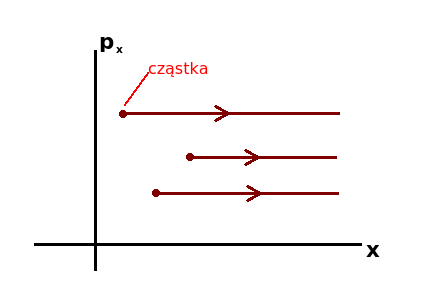
\includegraphics[scale=0.75] {obrazki/przestrzen_fazowa1.png}
\end{center}
\textbf{Uw.} Cząstki nie mogą być ułożone na 1 linii równoległej do osi pędowej, bo wtedy byłyby w 1 punkcie przestrzennym.
\end{verse}
\subsubsection{Opis gruboziarnisty}
Problem: potrzeba 2N warunków brzegowych.
Rozwiązanie: opis grupoziarnisty:\\
Wybierzmy element objętości przestrzeni $\mu$ wokół punktu L o objętości $[|\Delta \r_l|]^3$:
\begin{center}$dim[\mu]=2$\\
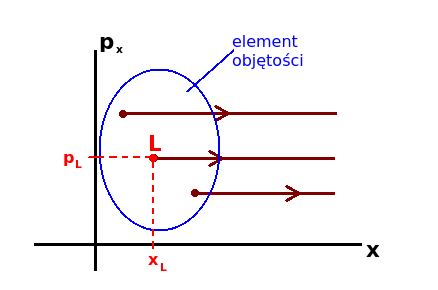
\includegraphics[scale=0.75] {obrazki/przestrzen_fazowa2.png}
\end{center}
Jeśli punkt:
\begin{equation} (\r_L,\p_L)\epsilon\mu~ \nonumber \end{equation}
wtedy element objętości:
\begin{equation}\Delta\omega_L=\Delta\r_L\Delta\p_L\end{equation}
przy czym wymiar elementu objętości jest rzędu długości, po której średniowaliśmy na poprzednich wykładach:
\begin{equation}|\Delta\r_L\sim L\sim 100nm\end{equation}
W kostce o takich rozmiarach liczba cząstek wynosi:
\begin{equation}[|\Delta\r_L|]^3[n_0 cm^{-3}]=[10^{-5}cm]^3[3\cdot10^{19}cm^{-3}]=3\cdot 10^4 \text{cząstek}\nonumber\end{equation}
Opis ten nazywamy opisem gruboziarnistym, ponieważ każdy element objętości dobieramy sobie dowolnie.

\subsection{Funkcja rozkładu gęstości prawdopodobieństwa}
\subsubsection{Definicja}
Wprowadźmy funkcję pomocniczą:
\begin{center}$\f$\end{center}
Żądamy, by była ona klasy $C^0[\mu]$, czyli by była ciągła w przestrzeni $\mu$.
Wyrażenie:
\begin{equation}\f\Delta\omega_L\end{equation}
opisuje liczbę cząstek w objętości $\Delta\omega_L$, w której położenia i prędkości zmieniają się zgodnie z rozkładem f.\\
Umówmy się, że:
\begin{equation}
\begin{cases} \sum_L f(\r_L,\p_L,t)\Delta\omega_L=\int d^3 r d^3 p\f \\ \int d^3r d^3p\f=N~\Rightarrow\text{f jest unormowana do liczby cząstek}\end{cases}
\end{equation}
Wówczas $\f$ jest \textbf{funkcją rozkładu gęstości prawdopodobieństwa}.
\subsubsection{Równanie kinetyczne dla tej funkcji}
\begin{itemize}
\item{Wyprowadzenie równania kinetycznego}\\
Zauważmy, że:
\begin{equation}f(\r,\p,t+dt)-\f \stackrel{\text{ciągłość f}, dt\rightarrow 0}{\simeq}\partial_t\f dt\end{equation}
gdzie
\begin{equation}\partial_t\equiv \frac{\partial}{\partial t}\end{equation}
W czasie dt położenie i pęd zmieniają się jak:
\begin{equation}d\r(t)=\dot{\r}(t)dt \end{equation}
\begin{equation} d\p(t)=\dot{\p}(t)dt \stackrel{\text{r.(\ref{RRuchu})}}{=}0\end{equation}
Wtedy:
\begin{equation}\f-f(\r+d\r,\p,t)\simeq -\dot{\r}(t)\nab{r}\f dt=-\frac{1}{m}\p(t)\nab{r}\f dt\end{equation}
i oczywiście:
\begin{equation}\f-f(\r,\p+d\p,t)\simeq -\dot{\p}(t)\nab{p}\f=0 \end{equation}
Zatem:
\begin{equation}\frac{d\f}{dt}=\partial_t\f+\frac{1}{m}\p(t)\cdot\nab{r}\f=0 \label{Rkinet}\end{equation} 
\textbf{Moja uwaga}: To zwykła "reguła łańcuchowa":
\begin{equation} \frac{d\f}{dt}=\frac{\partial\f}{\partial\r}\frac{\partial\r}{\partial t}+\frac{\partial\f}{\partial\p}\frac{\partial\p}{\partial t}+\frac{\partial\f}{\partial t}=\dot{r}(t)\nab{r}\f+0+\partial_t\f\end{equation}
Wiemy, że:
\begin{equation}mv(\p(t))=\p(t)~~ \Rightarrow ~~\vec{v}(\p(t))\equiv\v(\p)=\frac{1}{m}\p(t)\end{equation}
Wówczas równanie (\ref{Rkinet}) ma postać:
\begin{equation}\partial_t\f+\v(\p)\cdot\nab{r}\f=0\label{Rkinet2}\end{equation}
Powyższe równanie to \textbf{równanie kinetyczne}.
\item{Rozwiązanie równania kinetycznego}\\
Postulujemy rozwiązanie tego równania:
\begin{equation}\f=\Phi(\r-\v t,\p)\end{equation}
gdzie $\Phi$ to dowolna funkcja klasy $C^0[\mu]$.\\
Dowód, że jest to rozwiązanie:
\begin{verse}\textbf{ Ozn. }
\begin{equation} \vec{s}(t)=\r(t)-\v(t)\end{equation} \end{verse}
Wówczas kolejne części równania kinetycznego zyskują postać:
\begin{equation}\begin{cases} \Phi(\r-\v t,\p)~~\rightarrow ~~ \tilde{\Phi}(\vec{s}(t),\p) \\ 
\partial_t\Phi(\r(t)-\v t,\p)=\frac{\partial\vec{s}(t)}{\partial t}\nab{s}\tilde{\Phi}(\vec{s}(t),\p) \\ 
\nab{r}\Phi(\r(t)-\v t,\p)=\nab{r}\vec{s}t)\cdot\nab{s}\tilde{\Phi}(\vec{s}(t),\p)=\nab{s}\tilde{\Phi}(\vec{s}(t),\p) \end{cases}\end{equation}
Zatem równanie kinetyczne przyjmuje postać:
\begin{equation}\{-\v\cdot\nab{s}+\v\cdot\nab{s}\}\tilde{\Phi}(\vec{s}(t),\p)=0\end{equation}
Obie strony są równe, więc zaproponowana postać rozwiązania jest słuszna.
\end{itemize}
\subsubsection{Momenty funkcji rozkładu gęstości prawdopodobieństwa}
\begin{itemize}
\item {Zerowy moment}\\
\begin{equation}\int d^3p\f=n\arg\end{equation}
to zerowy moment funkcji rozkładu gęstości prawdpodobieństwa. Jest to jednocześnie rozkład brzegowy w przestrzeni położeniowej.
\item {Pierwszy moment}\\
Scałkujmy równanie kinetyczne (\ref{Rkinet2}) po pędzie:
\begin{equation}\partial_t\f+\v(\p)\cdot\nab{r}\f=0~~~~~~/\int d^3 \p\nonumber \end {equation}
\begin{equation}\partial_t n\arg+\int d^3\p ~\v(\p)\cdot\nab{r}\f=0 \nonumber\end{equation}
Pamiętamy, że wyszliśmy z hamiltonianu, w którym zmienne $\r,\p$ są niezależne (jesteśmy w przestrzeni $\mu$, zatem:
\begin{equation}\partial_t n\arg+\nab{r}\int d^3\p~\v(\p)\f=0 \nonumber\end{equation}
gdzie:
\begin{equation}\vec{j}\arg=\int d^3\p~\v(\p)\f\end{equation}
to pierwszy moemnt funkcji rozkładu gęstości prawdopodobieństwa. Jest on interpretowany jako prąd.
\end{itemize}
\subsubsection{Interpretacja}
\begin{itemize}
\item{Równanie kinetyczne jako równanie ciągłości}\\
Równanie kinetyczne wyrażone przez momenty ma postać:
\begin{equation}\partial_t n\arg+\nab{r}\j\arg=0\end{equation}
W ten sposób nadaliśmy równaniu kinetycznemu strukturę \textbf{równania ciągłości} ("nic nie może zginąć").
\item{Funkcja rozkładu gęstości prawdopodobieństwa wyrażona przez deltę Diraca}\\
Z definicji:
\begin{equation}\j\arg=\int d^3 p~\v(\p)\f\end{equation}
Z drugiej strony, w teorii Lorentza założyliśmy, że prąd cząsteczkowy ma postać:
\begin{equation}\j\arg=\sum_{i/1}^N\v_i(t)\delta(\r-\r_i(t))\end{equation}
Łącząc oba fakty, dostajemy:
\begin{equation}\f=const\cdot\sum_{i/1}^N\delta(\r-\r_i(t))\delta(\p)
\end{equation}
\textcolor{red}{!! Ale wtedy:
\begin{equation}\j\arg=const \int d^3p~\v(\p)\sum_{i/1}^N\delta(\r-\r_i(t))\delta(\p)\end{equation}
\begin{equation}\j\arg= const \int d^3p~\v(\p) \delta(\p) \sum_{i/1}^N\delta(\r-\r_i(t))
\end{equation}
\begin{equation}\j\arg=const~\v(\p=\vec{0}) \sum_{i/1}^N\delta(\r-\r_i(t))
\end{equation}}
Ile wynosi const.?
\begin{equation}\f=const\cdot\sum_{i/1}^N\delta(\r-\r_i(t))\delta(\p)~~~/\int d^3rd^3p \nonumber \end{equation}
\begin{equation}N=const\cdot N \nonumber \end{equation}
\begin{equation}const=1 \nonumber \end{equation}
Zatem:
\begin{equation}\f=\sum_{i/1}^N\delta(\r-\r_i(t))\delta(\p) \end{equation}
Ale:
\begin{equation}\r_i(t)=\r_{i0}+\frac{1}{m}\p_{i0}t=\r_{i0}+\v_{i0}t\end{equation}
zatem ostatecznie:
\begin{equation}\f=\sum_{i/1}^N\delta(\r-[\r_{i0}+\v{i0}t])\delta(\p) \end{equation}
\item{Interpretacja}\\
\begin{center}
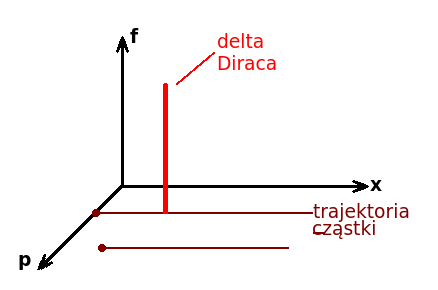
\includegraphics[scale=0.75]{obrazki/przestrzen_fazowa3.png}
\end{center}
Funkcja rozkładu gęstości prawdopodobieństwa przemieszcza się jako delta Diraca wzdłuż trajektorii fazowej w przestrzeni $\mu$ będącej rozwiązaniem kanonicznych równań Hamiltona.\\
\begin{verse}\textbf{Wn. }Założyliśmy brak zderzeń i dostaliśmy to:
\begin{center}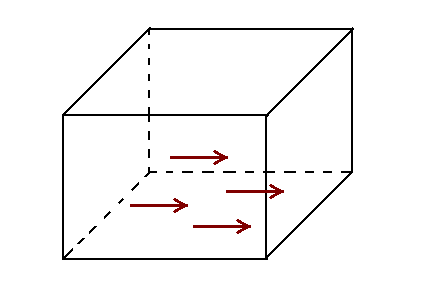
\includegraphics[scale=0.75]{obrazki/przestrzen_fazowa4.png}\end{center}
czyli prąd. \end{verse}
\end{itemize}

